% Generated by code/needham.py -- do not edit by hand.
\definecolor{qocA}{rgb}{0.00,0.45,0.70}
\definecolor{qocB}{rgb}{0.90,0.60,0.00}
\definecolor{qocC}{rgb}{0.00,0.62,0.45}
\definecolor{qocD}{rgb}{0.80,0.40,0.00}
\definecolor{qocE}{rgb}{0.80,0.60,0.70}
\definecolor{qocF}{rgb}{0.35,0.70,0.90}
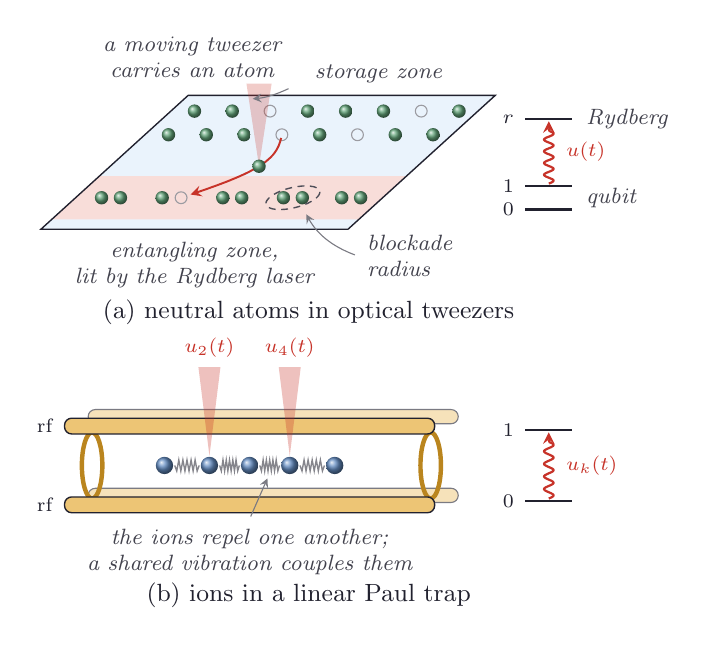
\begin{tikzpicture}[ink/.style={line width=0.9pt, ndInk}, faint/.style={line width=0.4pt, ndInk!35}, dashedink/.style={line width=0.5pt, ndInk!55, dash pattern=on 2.5pt off 2pt}, vec/.style={->, >=stealth, line width=1.2pt}, note/.style={font=\footnotesize\itshape, text=ndInk!85, align=center}, pointer/.style={->, >=stealth, line width=0.4pt, ndInk!60, shorten >=2pt, shorten <=1pt}, dot/.style={circle, fill=ndInk, inner sep=0pt, minimum size=3.4pt}, wash/.style={fill=ndSky, fill opacity=0.55}, every node/.style={text=ndInk}]
\definecolor{ndInk}{rgb}{0.13,0.13,0.18}
\definecolor{ndPaper}{rgb}{0.99,0.96,0.88}
\definecolor{ndSky}{rgb}{0.84,0.91,0.98}
\definecolor{ndRose}{rgb}{0.98,0.86,0.84}
\definecolor{ndBlue}{rgb}{0.13,0.36,0.66}
\definecolor{ndRed}{rgb}{0.78,0.20,0.16}
\definecolor{ndGold}{rgb}{0.88,0.62,0.10}
\definecolor{ndGreen}{rgb}{0.18,0.52,0.30}
\fill[ndSky, fill opacity=0.5] (0.000,4.100) -- (3.900,4.100) -- (5.770,5.800) -- (1.870,5.800) -- cycle;
\fill[ndRose, fill opacity=0.9] (0.138,4.225) -- (4.037,4.225) -- (4.643,4.775) -- (0.743,4.775) -- cycle;
\draw[ink, line width=0.5pt] (0.000,4.100) -- (3.900,4.100) -- (5.770,5.800) -- (1.870,5.800) -- cycle;
\shade[ball color=ndGreen!75] (1.950,5.600) circle (0.085);
\shade[ball color=ndGreen!75] (2.430,5.600) circle (0.085);
\draw[ndInk!45, line width=0.4pt] (2.910,5.600) circle (0.075);
\shade[ball color=ndGreen!75] (3.390,5.600) circle (0.085);
\shade[ball color=ndGreen!75] (3.870,5.600) circle (0.085);
\shade[ball color=ndGreen!75] (4.350,5.600) circle (0.085);
\draw[ndInk!45, line width=0.4pt] (4.830,5.600) circle (0.075);
\shade[ball color=ndGreen!75] (5.310,5.600) circle (0.085);
\shade[ball color=ndGreen!75] (1.620,5.300) circle (0.085);
\shade[ball color=ndGreen!75] (2.100,5.300) circle (0.085);
\shade[ball color=ndGreen!75] (2.580,5.300) circle (0.085);
\draw[ndInk!45, line width=0.4pt] (3.060,5.300) circle (0.075);
\shade[ball color=ndGreen!75] (3.540,5.300) circle (0.085);
\draw[ndInk!45, line width=0.4pt] (4.020,5.300) circle (0.075);
\shade[ball color=ndGreen!75] (4.500,5.300) circle (0.085);
\shade[ball color=ndGreen!75] (4.980,5.300) circle (0.085);
\shade[ball color=ndGreen!75] (0.770,4.500) circle (0.085);
\shade[ball color=ndGreen!75] (1.010,4.500) circle (0.085);
\shade[ball color=ndGreen!75] (1.540,4.500) circle (0.085);
\draw[ndInk!45, line width=0.4pt] (1.780,4.500) circle (0.075);
\shade[ball color=ndGreen!75] (2.310,4.500) circle (0.085);
\shade[ball color=ndGreen!75] (2.550,4.500) circle (0.085);
\shade[ball color=ndGreen!75] (3.080,4.500) circle (0.085);
\shade[ball color=ndGreen!75] (3.320,4.500) circle (0.085);
\shade[ball color=ndGreen!75] (3.820,4.500) circle (0.085);
\shade[ball color=ndGreen!75] (4.060,4.500) circle (0.085);
\draw[dashedink, ndInk!80] (3.500,4.500) -- (3.508,4.508) -- (3.516,4.516) -- (3.522,4.524) -- (3.528,4.531) -- (3.533,4.539) -- (3.536,4.547) -- (3.539,4.554) -- (3.541,4.561) -- (3.542,4.569) -- (3.542,4.576) -- (3.541,4.582) -- (3.539,4.589) -- (3.537,4.595) -- (3.533,4.601) -- (3.528,4.607) -- (3.523,4.612) -- (3.516,4.617) -- (3.509,4.622) -- (3.500,4.626) -- (3.491,4.631) -- (3.481,4.634) -- (3.471,4.638) -- (3.459,4.641) -- (3.447,4.643) -- (3.434,4.645) -- (3.421,4.647) -- (3.407,4.648) -- (3.392,4.649) -- (3.377,4.650) -- (3.361,4.650) -- (3.345,4.650) -- (3.328,4.649) -- (3.311,4.648) -- (3.294,4.646) -- (3.277,4.644) -- (3.259,4.642) -- (3.241,4.639) -- (3.223,4.636) -- (3.205,4.632) -- (3.187,4.629) -- (3.169,4.624) -- (3.151,4.620) -- (3.133,4.615) -- (3.115,4.610) -- (3.098,4.604) -- (3.081,4.598) -- (3.064,4.592) -- (3.048,4.586) -- (3.032,4.579) -- (3.016,4.572) -- (3.001,4.565) -- (2.987,4.558) -- (2.973,4.550) -- (2.960,4.543) -- (2.947,4.535) -- (2.935,4.528) -- (2.924,4.520) -- (2.914,4.512) -- (2.904,4.504) -- (2.896,4.496) -- (2.888,4.488) -- (2.881,4.480) -- (2.875,4.472) -- (2.870,4.465) -- (2.865,4.457) -- (2.862,4.450) -- (2.860,4.442) -- (2.858,4.435) -- (2.858,4.428) -- (2.858,4.421) -- (2.859,4.414) -- (2.862,4.408) -- (2.865,4.402) -- (2.869,4.396) -- (2.875,4.390) -- (2.881,4.385) -- (2.888,4.380) -- (2.895,4.376) -- (2.904,4.371) -- (2.914,4.368) -- (2.924,4.364) -- (2.935,4.361) -- (2.947,4.358) -- (2.959,4.356) -- (2.972,4.354) -- (2.986,4.352) -- (3.001,4.351) -- (3.016,4.350) -- (3.031,4.350) -- (3.047,4.350) -- (3.063,4.351) -- (3.080,4.352) -- (3.097,4.353) -- (3.115,4.355) -- (3.132,4.357) -- (3.150,4.359) -- (3.168,4.362) -- (3.186,4.366) -- (3.204,4.369) -- (3.222,4.374) -- (3.240,4.378) -- (3.258,4.383) -- (3.276,4.388) -- (3.293,4.393) -- (3.311,4.399) -- (3.327,4.405) -- (3.344,4.411) -- (3.360,4.418) -- (3.376,4.424) -- (3.391,4.431) -- (3.406,4.439) -- (3.420,4.446) -- (3.434,4.453) -- (3.447,4.461) -- (3.459,4.469) -- (3.470,4.476) -- (3.481,4.484) -- (3.491,4.492) -- (3.500,4.500);
\draw[->, >=stealth, line width=0.7pt, ndRed] (3.051,5.259) -- (3.047,5.246) -- (3.044,5.232) -- (3.040,5.219) -- (3.036,5.205) -- (3.031,5.192) -- (3.026,5.178) -- (3.021,5.164) -- (3.015,5.151) -- (3.008,5.137) -- (3.001,5.124) -- (2.994,5.110) -- (2.985,5.097) -- (2.976,5.083) -- (2.966,5.069) -- (2.956,5.056) -- (2.945,5.042) -- (2.932,5.029) -- (2.919,5.015) -- (2.905,5.002) -- (2.890,4.988) -- (2.874,4.975) -- (2.858,4.961) -- (2.840,4.947) -- (2.821,4.934) -- (2.801,4.920) -- (2.781,4.907) -- (2.759,4.893) -- (2.736,4.880) -- (2.713,4.866) -- (2.688,4.853) -- (2.662,4.839) -- (2.636,4.825) -- (2.608,4.812) -- (2.580,4.798) -- (2.550,4.785) -- (2.520,4.771) -- (2.489,4.758) -- (2.457,4.744) -- (2.424,4.731) -- (2.391,4.717) -- (2.356,4.703) -- (2.321,4.690) -- (2.285,4.676) -- (2.249,4.663) -- (2.212,4.649) -- (2.175,4.636) -- (2.137,4.622) -- (2.098,4.608) -- (2.059,4.595) -- (2.020,4.581) -- (1.981,4.568) -- (1.941,4.554) -- (1.901,4.541);
\fill[ndRed, fill opacity=0.25] (2.610,5.950) -- (2.930,5.950) -- (2.770,4.900) -- cycle;
\shade[ball color=ndGreen!75] (2.770,4.900) circle (0.085);
\node[note, anchor=south, align=center] (mv) at (1.920,5.900) {a moving tweezer\\ carries an atom};
\draw[pointer] (mv.south east) to[bend left=10] (2.620,5.750);
\node[note, anchor=south] at (4.288,5.830) {storage zone};
\node[note, anchor=north, align=center] at (1.950,4.060) {entangling zone,\\ lit by the Rydberg laser};
\node[note, anchor=north west, align=left] (br) at (4.020,4.150) {blockade\\ radius};
\draw[pointer] (br.west) to[bend left=20] (3.335,4.350);
\draw[ink] (6.150,4.350) -- ++(0.600,0);
\node[font=\scriptsize, anchor=east] at (6.130,4.350) {$\ket{0}$};
\draw[ink] (6.150,4.650) -- ++(0.600,0);
\node[font=\scriptsize, anchor=east] at (6.130,4.650) {$\ket{1}$};
\draw[ink] (6.150,5.500) -- ++(0.600,0);
\node[font=\scriptsize, anchor=east] at (6.130,5.500) {$\ket{r}$};
\draw[line width=0.8pt, ndRed] (6.450,4.680) -- (6.461,4.684) -- (6.471,4.688) -- (6.481,4.693) -- (6.489,4.697) -- (6.497,4.701) -- (6.503,4.705) -- (6.507,4.709) -- (6.509,4.714) -- (6.510,4.718) -- (6.509,4.722) -- (6.506,4.726) -- (6.501,4.731) -- (6.494,4.735) -- (6.486,4.739) -- (6.477,4.743) -- (6.468,4.747) -- (6.457,4.752) -- (6.446,4.756) -- (6.436,4.760) -- (6.426,4.764) -- (6.416,4.768) -- (6.408,4.773) -- (6.401,4.777) -- (6.396,4.781) -- (6.392,4.785) -- (6.390,4.790) -- (6.390,4.794) -- (6.392,4.798) -- (6.396,4.802) -- (6.401,4.806) -- (6.408,4.811) -- (6.416,4.815) -- (6.426,4.819) -- (6.436,4.823) -- (6.446,4.827) -- (6.457,4.832) -- (6.468,4.836) -- (6.477,4.840) -- (6.486,4.844) -- (6.494,4.849) -- (6.501,4.853) -- (6.506,4.857) -- (6.509,4.861) -- (6.510,4.865) -- (6.509,4.870) -- (6.507,4.874) -- (6.503,4.878) -- (6.497,4.882) -- (6.489,4.886) -- (6.481,4.891) -- (6.471,4.895) -- (6.461,4.899) -- (6.450,4.903) -- (6.439,4.908) -- (6.429,4.912) -- (6.419,4.916) -- (6.411,4.920) -- (6.403,4.924) -- (6.397,4.929) -- (6.393,4.933) -- (6.391,4.937) -- (6.390,4.941) -- (6.391,4.945) -- (6.394,4.950) -- (6.399,4.954) -- (6.406,4.958) -- (6.414,4.962) -- (6.423,4.967) -- (6.432,4.971) -- (6.443,4.975) -- (6.454,4.979) -- (6.464,4.983) -- (6.474,4.988) -- (6.484,4.992) -- (6.492,4.996) -- (6.499,5.000) -- (6.504,5.004) -- (6.508,5.009) -- (6.510,5.013) -- (6.510,5.017) -- (6.508,5.021) -- (6.504,5.026) -- (6.499,5.030) -- (6.492,5.034) -- (6.484,5.038) -- (6.474,5.042) -- (6.464,5.047) -- (6.454,5.051) -- (6.443,5.055) -- (6.432,5.059) -- (6.423,5.063) -- (6.414,5.068) -- (6.406,5.072) -- (6.399,5.076) -- (6.394,5.080) -- (6.391,5.085) -- (6.390,5.089) -- (6.391,5.093) -- (6.393,5.097) -- (6.397,5.101) -- (6.403,5.106) -- (6.411,5.110) -- (6.419,5.114) -- (6.429,5.118) -- (6.439,5.122) -- (6.450,5.127) -- (6.461,5.131) -- (6.471,5.135) -- (6.481,5.139) -- (6.489,5.144) -- (6.497,5.148) -- (6.503,5.152) -- (6.507,5.156) -- (6.509,5.160) -- (6.510,5.165) -- (6.509,5.169) -- (6.506,5.173) -- (6.501,5.177) -- (6.494,5.181) -- (6.486,5.186) -- (6.477,5.190) -- (6.468,5.194) -- (6.457,5.198) -- (6.446,5.203) -- (6.436,5.207) -- (6.426,5.211) -- (6.416,5.215) -- (6.408,5.219) -- (6.401,5.224) -- (6.396,5.228) -- (6.392,5.232) -- (6.390,5.236) -- (6.390,5.240) -- (6.392,5.245) -- (6.396,5.249) -- (6.401,5.253) -- (6.408,5.257) -- (6.416,5.262) -- (6.426,5.266) -- (6.436,5.270) -- (6.446,5.274) -- (6.457,5.278) -- (6.468,5.283) -- (6.477,5.287) -- (6.486,5.291) -- (6.494,5.295) -- (6.501,5.299) -- (6.506,5.304) -- (6.509,5.308) -- (6.510,5.312) -- (6.509,5.316) -- (6.507,5.321) -- (6.503,5.325) -- (6.497,5.329) -- (6.489,5.333) -- (6.481,5.337) -- (6.471,5.342) -- (6.461,5.346) -- (6.450,5.350);
\draw[->, >=stealth, line width=0.8pt, ndRed] (6.450,5.350) -- (6.450,5.470);
\node[font=\scriptsize, text=ndRed, anchor=west] at (6.550,5.090) {$u(t)$};
\node[note, anchor=west] at (6.800,5.500) {Rydberg};
\node[note, anchor=west] at (6.800,4.500) {qubit};
\node[font=\small] at (3.400,3.050) {(a) neutral atoms in optical tweezers};
\filldraw[ndGold!30!white, draw=ndInk!60, line width=0.4pt, rounded corners=0.9mm] (0.600,1.630) rectangle (5.300,1.810);
\filldraw[ndGold!30!white, draw=ndInk!60, line width=0.4pt, rounded corners=0.9mm] (0.600,0.630) rectangle (5.300,0.810);
\draw[ndGold!80!ndInk, line width=1.6pt] (0.650,1.100) ellipse (0.13 and 0.42);
\draw[ndGold!80!ndInk, line width=1.6pt] (4.950,1.100) ellipse (0.13 and 0.42);
\draw[line width=0.5pt, ndInk!55] (1.699,1.100) -- (1.725,1.030) -- (1.751,1.170) -- (1.777,1.030) -- (1.803,1.170) -- (1.829,1.030) -- (1.855,1.170) -- (1.881,1.030) -- (1.907,1.170) -- (1.933,1.030) -- (1.958,1.170) -- (1.984,1.030) -- (2.010,1.100);
\draw[line width=0.5pt, ndInk!55] (2.270,1.100) -- (2.291,1.030) -- (2.312,1.170) -- (2.333,1.030) -- (2.354,1.170) -- (2.374,1.030) -- (2.395,1.170) -- (2.416,1.030) -- (2.437,1.170) -- (2.458,1.030) -- (2.478,1.170) -- (2.499,1.030) -- (2.520,1.100);
\draw[line width=0.5pt, ndInk!55] (2.780,1.100) -- (2.801,1.030) -- (2.822,1.170) -- (2.842,1.030) -- (2.863,1.170) -- (2.884,1.030) -- (2.905,1.170) -- (2.926,1.030) -- (2.946,1.170) -- (2.967,1.030) -- (2.988,1.170) -- (3.009,1.030) -- (3.030,1.100);
\draw[line width=0.5pt, ndInk!55] (3.290,1.100) -- (3.316,1.030) -- (3.342,1.170) -- (3.367,1.030) -- (3.393,1.170) -- (3.419,1.030) -- (3.445,1.170) -- (3.471,1.030) -- (3.497,1.170) -- (3.523,1.030) -- (3.549,1.170) -- (3.575,1.030) -- (3.601,1.100);
\shade[ball color=ndBlue!70] (1.569,1.100) circle (0.110);
\shade[ball color=ndBlue!70] (2.140,1.100) circle (0.110);
\shade[ball color=ndBlue!70] (2.650,1.100) circle (0.110);
\shade[ball color=ndBlue!70] (3.160,1.100) circle (0.110);
\shade[ball color=ndBlue!70] (3.731,1.100) circle (0.110);
\filldraw[ndGold!60!white, draw=ndInk, line width=0.5pt, rounded corners=0.9mm] (0.300,1.500) rectangle (5.000,1.700);
\filldraw[ndGold!60!white, draw=ndInk, line width=0.5pt, rounded corners=0.9mm] (0.300,0.500) rectangle (5.000,0.700);
\fill[ndRed, fill opacity=0.3] (2.000,2.350) -- (2.280,2.350) -- (2.140,1.220) -- cycle;
\node[font=\scriptsize, text=ndRed, anchor=south] at (2.140,2.350) {$u_{2}(t)$};
\fill[ndRed, fill opacity=0.3] (3.020,2.350) -- (3.300,2.350) -- (3.160,1.220) -- cycle;
\node[font=\scriptsize, text=ndRed, anchor=south] at (3.160,2.350) {$u_{4}(t)$};
\node[note, anchor=north, align=center] (sp) at (2.650,0.420) {the ions repel one another;\\ a shared vibration couples them};
\draw[pointer] (sp.north) -- (2.905,1.000);
\node[font=\scriptsize, anchor=east] at (0.270,1.600) {rf};
\node[font=\scriptsize, anchor=east] at (0.270,0.600) {rf};
\draw[ink] (6.150,0.650) -- ++(0.600,0);
\node[font=\scriptsize, anchor=east] at (6.130,0.650) {$\ket{0}$};
\draw[ink] (6.150,1.550) -- ++(0.600,0);
\node[font=\scriptsize, anchor=east] at (6.130,1.550) {$\ket{1}$};
\draw[line width=0.8pt, ndRed] (6.450,0.680) -- (6.461,0.685) -- (6.471,0.689) -- (6.481,0.694) -- (6.489,0.698) -- (6.497,0.703) -- (6.503,0.707) -- (6.507,0.712) -- (6.509,0.716) -- (6.510,0.721) -- (6.509,0.725) -- (6.506,0.730) -- (6.501,0.734) -- (6.494,0.739) -- (6.486,0.743) -- (6.477,0.748) -- (6.468,0.752) -- (6.457,0.757) -- (6.446,0.762) -- (6.436,0.766) -- (6.426,0.771) -- (6.416,0.775) -- (6.408,0.780) -- (6.401,0.784) -- (6.396,0.789) -- (6.392,0.793) -- (6.390,0.798) -- (6.390,0.802) -- (6.392,0.807) -- (6.396,0.811) -- (6.401,0.816) -- (6.408,0.820) -- (6.416,0.825) -- (6.426,0.829) -- (6.436,0.834) -- (6.446,0.838) -- (6.457,0.843) -- (6.468,0.848) -- (6.477,0.852) -- (6.486,0.857) -- (6.494,0.861) -- (6.501,0.866) -- (6.506,0.870) -- (6.509,0.875) -- (6.510,0.879) -- (6.509,0.884) -- (6.507,0.888) -- (6.503,0.893) -- (6.497,0.897) -- (6.489,0.902) -- (6.481,0.906) -- (6.471,0.911) -- (6.461,0.915) -- (6.450,0.920) -- (6.439,0.925) -- (6.429,0.929) -- (6.419,0.934) -- (6.411,0.938) -- (6.403,0.943) -- (6.397,0.947) -- (6.393,0.952) -- (6.391,0.956) -- (6.390,0.961) -- (6.391,0.965) -- (6.394,0.970) -- (6.399,0.974) -- (6.406,0.979) -- (6.414,0.983) -- (6.423,0.988) -- (6.432,0.992) -- (6.443,0.997) -- (6.454,1.002) -- (6.464,1.006) -- (6.474,1.011) -- (6.484,1.015) -- (6.492,1.020) -- (6.499,1.024) -- (6.504,1.029) -- (6.508,1.033) -- (6.510,1.038) -- (6.510,1.042) -- (6.508,1.047) -- (6.504,1.051) -- (6.499,1.056) -- (6.492,1.060) -- (6.484,1.065) -- (6.474,1.069) -- (6.464,1.074) -- (6.454,1.078) -- (6.443,1.083) -- (6.432,1.088) -- (6.423,1.092) -- (6.414,1.097) -- (6.406,1.101) -- (6.399,1.106) -- (6.394,1.110) -- (6.391,1.115) -- (6.390,1.119) -- (6.391,1.124) -- (6.393,1.128) -- (6.397,1.133) -- (6.403,1.137) -- (6.411,1.142) -- (6.419,1.146) -- (6.429,1.151) -- (6.439,1.155) -- (6.450,1.160) -- (6.461,1.165) -- (6.471,1.169) -- (6.481,1.174) -- (6.489,1.178) -- (6.497,1.183) -- (6.503,1.187) -- (6.507,1.192) -- (6.509,1.196) -- (6.510,1.201) -- (6.509,1.205) -- (6.506,1.210) -- (6.501,1.214) -- (6.494,1.219) -- (6.486,1.223) -- (6.477,1.228) -- (6.468,1.232) -- (6.457,1.237) -- (6.446,1.242) -- (6.436,1.246) -- (6.426,1.251) -- (6.416,1.255) -- (6.408,1.260) -- (6.401,1.264) -- (6.396,1.269) -- (6.392,1.273) -- (6.390,1.278) -- (6.390,1.282) -- (6.392,1.287) -- (6.396,1.291) -- (6.401,1.296) -- (6.408,1.300) -- (6.416,1.305) -- (6.426,1.309) -- (6.436,1.314) -- (6.446,1.318) -- (6.457,1.323) -- (6.468,1.328) -- (6.477,1.332) -- (6.486,1.337) -- (6.494,1.341) -- (6.501,1.346) -- (6.506,1.350) -- (6.509,1.355) -- (6.510,1.359) -- (6.509,1.364) -- (6.507,1.368) -- (6.503,1.373) -- (6.497,1.377) -- (6.489,1.382) -- (6.481,1.386) -- (6.471,1.391) -- (6.461,1.395) -- (6.450,1.400);
\draw[->, >=stealth, line width=0.8pt, ndRed] (6.450,1.400) -- (6.450,1.520);
\node[font=\scriptsize, text=ndRed, anchor=west] at (6.550,1.100) {$u_k(t)$};
\node[font=\small] at (3.400,-0.550) {(b) ions in a linear Paul trap};
\end{tikzpicture}
